% documento de exemplo modificado a partir do modelo original para teses e dissertações do 
% Programa de Pós-Graduaçãoe em Ciência da Comptuação da UFMG - PPGCC-UFMG, onde as teses 
% foram substituídas por TCCs
\documentclass[proposal]{ppgccufmg} % utilizem [tcc] para a monografia final ou [proposal] para projeto de TCC

\usepackage[brazil]{babel}      % se o documento for em português, OU
%\usepackage[latin1]{inputenc}
\usepackage[utf8]{inputenc}
\usepackage[T1]{fontenc} 
\usepackage{graphicx}
\usepackage[a4paper,
  portuguese,
  bookmarks=true,
  bookmarksnumbered=true,
  linktocpage,
  colorlinks,
  citecolor=black,
  urlcolor=blue,
  linkcolor=blue,
  filecolor=black,
  ]{hyperref}
%\usepackage[round]{natbib}
\usepackage[plain]{natbib}
%\usepackage[style=abnt]{biblatex}
%\addbibresource{6-bibfile.bib}  


\begin{document}

% O comando a seguir, \ppgccufmg, provê todas as informações relevantes para a
% classe ppgccufmg. Por favor, consulte a documentação para a descrição de
% cada chave.

% Um exemplo para documentos em português é apresentado a seguir:
\ppgccufmg{
  title={Estudo de viabilidade de um sistema de identificação de chamadas falsas em chamadas de emergência},
  authorrev={Viana, Robert Cristiano Almeida},
  %cutter={D1234p},   % dados que futuramente serão utilizados pela biblioteca
  %cdu={519.6*82.10}, % dados que futuramente serão utilizados pela biblioteca
  university={Instituto Federal do Norte de Minas Gerais},
  campus={Montes Claros},
  coursetype = {Bacharelado},
  course={Ciência da Computação},
  address={Montes Claros},
  date={2019-04},
  keywords={Inteligência Artificial, Chamadas emergenciais, Classificação de texto, Redes Neurais, Processamento de Linguagem Natural},
  advisor={Luciana Balieiro Cosme},
%  approval={img/approvalsheet.eps},
  abstract={Resumo}{0-Resumo},
  abstract=[english]{Abstract}{0-Abstract},
  %dedication={dedicatoria},
  %ack={agradecimentos},
  epigraphtext={If it wasn't hard, everyone would do it. It's the hard that makes it great}{Tom Hanks},
}

\usepackage{array}
\newcolumntype{L}[1]{>{\raggedright\let\newline\\\arraybackslash\hspace{0pt}}m{#1}}
\newcolumntype{C}[1]{>{\centering\let\newline\\\arraybackslash\hspace{0pt}}m{#1}}
\newcolumntype{R}[1]{>{\raggedleft\let\newline\\\arraybackslash\hspace{0pt}}m{#1}}

% Inclua cada capítulo em um arquivo separado para melhorar a organização
\chapter{Introdução}
Com o objetivo de ampliar, regulamentar e aumentar a eficiência dos serviços de urgência no Brasil, o Ministério da Saúde publicou duas portarias em 2003, a GM/MS nº 1863 e a GM/MS nº 1864 que instituíram, respectivamente, a Política Nacional de Atenção às Urgências e o componente pré-hospitalar móvel, por meio da implantação do Serviço de Atendimento Móvel de Urgência (SAMU), disponível através do número telefônico $192$, como também os serviços de urgência associados, em todo o território nacional \citep{p1863, p1864}. A implantação desses projetos mostrou grandes impactos positivos \citep{VIEIRA2008, MACHADO2011, MINAYO2008}. 

Contudo, também surgiram novos problemas e desafios. Um dos principais encontrados são as chamadas falsas ou trotes, no qual o individuo entra em contato com a unidade de atendimento e relata uma situação inexistente, que quando não identificado pelo atendente, pode resultar em deslocamentos desnecessários de unidades e recursos ao local do chamado. Outra situação comum, são as chamadas com categorização não emergencial, em que a população procura por orientações, tais como números de outros serviços, locais e endereços. 

O grande problema dessas ligações é que elas ocupam a linha emergencial e gastam recursos, gerando transtornos para os serviços de emergência. Este é um fator tão preocupante que, quando escasso de recursos, uma pessoa que realmente necessite de atendimento pode sofrer sequelas, ou até mesmo não resistir.

Além desses riscos, uma mobilização indevida de recursos, seja ela de pessoas, viaturas, ambulâncias, carros de combate a incêndio e principalmente tempo, geram também prejuízos financeiros ao Estado. E esses recursos que poderiam ser investidos em outros setores, como educação, infraestrutura ou segurança, por exemplo, acabam tendo que ser remanejados, resultando diretamente na qualidade de vida da sociedade que paga impostos.

O ato do trote aos serviços de emergência é um crime previsto no Código Penal brasileiro. Segundo o Art. nº 340 do Código Penal \citep{cp340}, "Provocar a ação de autoridade, comunicando-lhe a ocorrência de crime ou de contravenção que sabe não se ter verificado", quando identificado o autor, o mesmo pode ser detido por um período de um a seis meses ou multado. Com uma análise cautelosa ao artigo, percebe-se que o mesmo não abrange a comunicação falsa de situações de emergência que motivem o acionamento do Serviço de Atendimento Móvel de Urgência (SAMU) ou corpo de bombeiros, e sim somente nos casos em que há relato de infrações penais. Como relatado por \cite{peixoto2015combate}, existem outros artigos e projetos de leis que poderiam ajudar a punir tal ato, mas devido a sua natureza, talvez não sejam a melhor opção para o problema. 

Embora que, grande parte dos autores de chamados falsos são crianças e adolescentes, e por serem menores de idade, são inalcançáveis pelo direito penal, em razão de sua inimputabilidade, o problema se encontra em chamadas falsas iniciadas por adultos, pois o conteúdo dessas mensagens tendem a serem mais próximas de uma ocorrência real. Dificultando assim, a identificação de ser uma chamada falsa pelo atendente.

Após uma consulta na literatura disponível, não foram encontrados muitos resultados que visam identificar tais chamadas emergenciais falsas. O que nos levar a crer que, por ser uma área com pouca visibilidade, exista outros fatores que influenciam tão baixo investimento em pesquisas e soluções. Um desses fatores é que o conteúdo dessas ligações são sensíveis a privacidade e sujeitos a análise por um conselho de ética. Sendo essa, uma grande barreira e um processo burocrático para o desencadeamento de pesquisas. Além disso, os gestores (responsáveis pelos dados) podem se sentir menos dispostos a disponibilizar dados anônimos para pesquisas devido a falta de divulgação de resultados positivos.

Existem poucas bases de dados públicas disponíveis para realizações de experimentos e prova de metodologias, que seriam capazes de solucionar tal problema. E ainda dentre tais bases, a maioria está disponível no idioma inglês, e os dados que são disponibilizados são rasos, carecendo de detalhes e proporcionando pouco espaço para uma exploração aprofundada.

\section{Motivação}
Devido à proporção do problema, os atendentes do Centro Integrado de Operações de Segurança Pública (CIOSP) do governo de Mato Grosso, responsáveis estes pelo atendimento e despacho das chamadas emergenciais, receberam uma capacitação para identificar suspeitas de trote. Embora não seja possível bloquear todas ligações indevidas, a triagem ajuda a amenizar os prejuízos \citep{govMatoGrosso2016}.

Segundo um estudo apontado pela Consultoria Legislativa do Senado, estima-se que o custo gerado por trotes aos serviços de emergência no Brasil, tais como o Serviço de Atendimento Móvel de Urgência (SAMU), Corpo de Bombeiros (CB) e Polícia Militar (PM), chega a R\$ $1$ bilhão por ano. Esse levantamento foi apurado pela PM do estado do Amapá, onde eles avaliaram que a cada deslocamento para um atendimento emergencial incompleto, gera um custo aproximado de R\$ $500$ \citep{globo2014trotes, peixoto2015combate}.

\section{Objetivos}

\section{Estrutura do trabalho}


\chapter{Conceitos Básicos}
Nesta seção, serão explorados alguns fundamentos básicos para compreender, passo a passo, como será conduzida a metodologia proposta. Primeiramente, introduz-se o problema da classificação de dados. Logo após esse conceito, descreve-se como exemplos de técnicas de categorização de dados, as Redes Neurais Artificiais (RNA) e o K-vizinhos mais próximos. Por fim, é apresentado uma introdução ao Processamento de Linguagem Natural (PLN), dando enfase a um sub-conceito muito valioso para os objetivos deste trabalho, que é a classificação de texto.

\section{Processamento de linguagem natural}
O processamento de linguagem natural (PLN) têm como objetivo tratar os mais diversos aspectos presentes dentro da comunicação humana, tais como sons, palavras, sentenças e discursos, levando em consideração os seus formatos, referências, estruturas, significados, contextos e aplicações. Embora exista outros animais que possuem um vocabulário com centenas de sinais, tais como os elefantes e os golfinhos, somente os seres humanos possuem a capacidade de se comunicar, de forma confiável, em um número ilimitado de mensagens qualitativamente diferentes, sobre um tema qualquer \citep{russell1994inteligencia, gonzalez2003recuperaccao}.

Hoje em dia, com o constante crescimento da rede mundial de computadores, possibilitou o acesso a enumeras páginas de informações na \textit{Web}, no qual quase todas elas estão em um formato de linguagem natural. Entretanto, disponibilidade não significa fácil acesso à informação. Para uma máquina adquirir tal conhecimento, ela precisa ser treinada, de forma exaustiva, para compreender as complexas, e muitas vezes ambíguas, linguagens em que os seres humanos se comunicam.

Segundo \cite{russell1994inteligencia}, as linguagens naturais, tais como o português e o espanhol, não podem ser caracterizadas como um conjunto de sentenças definitivas, pois de acordo com o contexto em que for definida uma sentença de alguma dessas linguagens, ela pode possuir inúmeras interpretações diferentes. Portanto, convém definir um modelo de linguagem natural como uma distribuição de probabilidade sobre sentenças. Existe um famoso ditado popular brasileiro que diz "para um bom entendedor, meia palavra basta", o que pode ser comumente aplicado para nós humanos, que possuímos uma espécie de dispositivo de especialização para aquisição de linguagens \citep{chomsky2014aspects}. Já que meia palavra basta, pode-se concluir que uma sentença de uma linguagem natural não é sempre aleatória, e que sim possui algum grau de previsibilidade e correlação entre a escolha das palavras. Portanto, nos leva a acreditar que palavras similares estejam presentes no mesmo contexto.

O PLN consiste no emprego de um conjunto de técnicas computacionais para aprender, entender e reproduzir uma linguagem natural. No processo de tradução do significado, tratamento de ambiguidade e entre outros desafios, o PLN pode utilizar de conhecimentos linguísticos e métodos estatísticos para resolvê-los. Para isso, em geral é necessário que as palavras
sejam tratadas e transformadas em uma representação adequada, para enfim serem utilizadas por algoritmos de classificação. Por exemplo, considere uma análise sobre dois textos semelhantes A e B, no qual desconfia-se que exista possibilidade de plágio. Com o uso de um pré-processamento, seria possível filtrar os textos para remover \textit{Stopwords}, que são palavras funcionais, tais como artigos, preposições e conetivos, advindas de uma lista pré definida, que quando analisadas individualmente não possuem grande relevância para o contexto. Após tal pré-processamento, seria possível aplicar algum método de distância mínima de edição, tal como a distância Levenshtein que responderia o quão semelhante os textos são, através de uma análise sobre a quantidade de operações que seriam necessárias para transformar o texto A no texto B, ou vice e versa. Embora que, seja um método bastante custoso, devido ao fato de comparar cada caractere entre os textos, é um método muito útil para comparar a semelhança de dois textos e possui diversas aplicações, tais como nos algoritmos de verificação ortográfica automática, como também em outras áreas, como na biologia computacional quando é necessário analisar sequências biológicas.

Uma das tarefas possíveis no PLN é a classificação de texto. Para compreender melhor o processo de aplicação de conhecimentos linguísticos para essa tarefa, é apresentado a seguir uma seção sobre classificação de texto.

\subsection{Classificação de texto}
Segundo \cite{aggarwal2014data} um dos principais desafios encontrados durante o processo de classificação de texto é sobre o tamanho dos dados tratados, que podem variar de algumas poucas dezenas para milhões de palavras. Esses dados se encontram, quase sempre, de maneira esparsa, ou seja, possuindo baixa frequência de uso. Por outro lado, têm-se muitas vezes uma alta frequência de dados não úteis para tratamento, como as \textit{Stopwords}.

É comum também, dependendo do contexto ou de como obteve-se o texto, que exista palavras com o mesmo significado, erros ortográficos ou até mesmo erros de codificação. Logo, muitas vezes é necessário uma etapa de normalização do texto. Normalizar um texto significa, segundo \citep{martin2018speech}, converte-lo dê forma conveniente à um formato padrão, que facilite as manipulações sobre os dados. Exemplos de sub-etapas da normalização são: \textit{tokenization} e \textit{lemmatization}. 

Na \textit{tokenization}, deseja-se separar as palavras contidas em um texto, de maneira que elas fiquem isoladas. Por exemplo, na frase "fui ao Rio de Janeiro", resultaria em 5 \textit{tokens} distintos: "fui", "ao", "Rio", "de", "Janeiro". Contudo, uma separação em \textit{tokens} por somente o uso do espaçamento em branco, nem sempre representa o contexto da frase, pois como no exemplo "fui ao Rio de Janeiro", Rio de Janeiro não deve ser tratado como três \textit{tokens} distintos, e sim como um único \textit{token}, que no caso representa a cidade ou estado brasileiro. Em algumas linguagens naturais, nem todas palavras possuem espaço entre si, como é o caso da linguagem mandarim, utilizado majoritariamente no norte e sudoeste da China, o que vem a ser um mais um empecilho no processo de \textit{tokenization}. 

A etapa de \textit{lemmatization}, é o processo, efetivamente, de deflexionar uma palavra para determinar o seu lema. Por exemplo, as palavras gato, gata, gatos, gatas são todas formas do mesmo lema: gato. Igualmente, as palavras estudou, estudava, estudaria, estudará, são do mesmo lema: estudar. A lematização é útil quando deseja-se ver os usos de palavras em contextos sem importância das flexões, como também para a criação e uso de índices ou na investigação linguística. Por poder se tornar um processo custoso, dependendo da quantidade de dados, uma alternativa mais barata acaba sendo mais viável nesses cenários. Surgindo então o conceito de uma análise morfológica, chamada \textit{stemming}.

No \textit{stemming}, deseja-se reduzir as palavras flexionadas, ou às vezes derivadas, ao seu tronco, base ou raiz, cortando assim caracteres dos seus sufixos. Por exemplo, a stemização das palavras estudou, estudava, estudaria, estudará, será "estud", visto que é o prefixo comum e redutível por todos. Um dos algoritmos mais conhecidos para \textit{stemming} é o Porter, proposto por \citep{porter1980algorithm}. Se por um lado, facilita a identificação de variantes para um mesmo lema e possui o potencial de lidar com palavras desconhecidas, transformando-as em uma semelhante conhecida, pelo outro lado, a utilização deste método pode gerar erros de interpretação, tanto quando ele corta demais as palavras, como também quando ele não corta o suficiente, permanecendo a ambiguidade.

Além de uma etapa de normalização dos dados, uma etapa para extração e seleção de características é essencial, e pode gerar benefícios como: redução da dimensão do problema, que por sua vez aumenta a velocidade de execução do algoritmo; redução na quantidade total de características; aumento na precisão de predição e acerto; e facilitar a visualização dos dados.

Uma vez escolhido um conjunto de características, é possível aplicar algumas técnicas de classificação de texto, inclusive duas das que já foram abordadas aqui, as redes neurais artificiais e o k-vizinhos mais próximos, nos quais apresentam uma precisão superior a 98\% quando aplicados ao problema de identificação de \textit{e-mail spam} \citep{russell1994inteligencia}.

A classificação ou categorização de texto é portanto a tarefa de, dado algum tipo de texto, decidir a qual conjunto predefinido de classes o mesmo pertence. Por exemplo, decidir a qual linguagem pertence uma sentença ou identificar se um texto de uma chamada de emergência é falsa ou não, são exemplos de classificação de texto.

\section{Classificação de dados}
Classificação de dados é um problema que abrange inúmeras aplicações em diversos tipos de cenários no nosso dia a dia, tais como diagnóstico de doenças, identificação de objetos em fotos e vídeos, categorização de seres vivos e espécies, dentre outros. Esse problema é um dos tópicos mais ativos na área de aprendizado de máquina. Classificar dados consiste em determinar um rótulo ou classe para um objeto, baseado em um conjunto de características extraídas do mesmo \citep{duda1973pattern,bishop2006pattern}. 

Em geral, cada dado é classificado como pertencente a uma única classe ou categoria. Essa forma de classificação é denominada classificação de rótulo único. Por outro lado, se houver mais uma forma de rotular a mesma entrada, então dá-se o nome de classificação de multi-rótulo. 

Formalmente, o processo de classificação consiste em: um conjunto de $i$ entradas $X = \{X_1,...,X_i\}$, um conjunto de $n$ classes $C = \{c_1,...,c_n\}$, tal que $n \geq 2$, e um conjunto de treinamento $Y = \{(X_1, \{c_1,...,c_j\}),...,(X_i, \{c_n,...,c_k\})\}$, no qual cada entrada $X_i$ é categorizada por uma ou mais classes $c_i$. O objetivo geral de um classificador é aprender, através de seu conjunto de treinamento $Y$, uma possível correlação entre os atributos das entradas com suas classes, de tal forma que para uma entrada $X' = \{X'_1,...,X'_i\}$ que não possua rótulo $c$ qualquer, seja possível classificá-la.

Para ilustrar o processo de classificação de dados, considere o problema da flor de Iris. Nesse problema, existe um conjunto de flores do gênero Iris que podem ser rotuladas de uma das três maneiras: do tipo setosa, virgínica ou versicolor. Partindo desse ponto, o objetivo é determinar a qual grupo uma determinada flor pertence baseado nas medidas de sépalas e pétalas da mesma. A Figura \ref{fig:irisExample} ilustra o processo de classificação. Inicialmente as informações específicas sobre as sépalas e pétalas devem ser extraídas em um pré-processamento. Em seguida tais medidas são processadas e suas características extraídas. Por fim, é realizada a classificação das flores. Neste exemplo os valores de $X$ serão as medidas de comprimento, largura das sépalas e pétalas e $C$ assumirá os rótulos setosa, virgínica e versicolor.

Em geral, existem diversos algoritmos para classificação de dados, em que cada um possui sua especificidade, vantagens e desvantagens. Neste trabalho, aborda-se o uso de duas técnicas clássicas para classificação de dados: Redes Neurais Artificiais (RNA) e K-vizinhos mais próximos (KNN).

\begin{figure}[ht!]
\caption{Processo de classificação de flores do gênero Iris}
\label{fig:irisExample}
\centering
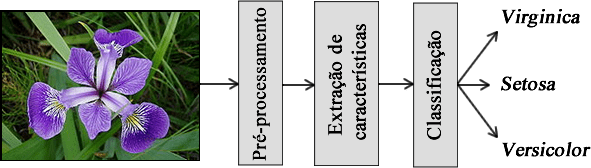
\includegraphics[scale=0.65]{img/irisExample.png}
{\fontsize{11pt}{\baselineskip}\selectfont
\\Fonte: \cite{pacheco2016agregaccao}
}
\end{figure}

\subsection{Redes neurais artificiais (RNA)}
O ser humano possui capacidades cognitivas extraordinárias e, desde o surgimento da computação, desejou-se projetar máquinas capazes de realizar tarefas inteligentes que, até então, somente eram  executadas por humanos. Os primeiros trabalhos desenvolvidos nessa área foram: um neurônio apresentado por \cite{mcculloch1943logical}, usado posteriormente como base para a concepção do  \textit{Perceptron} por \cite{rosenblatt1958perceptron} e um neurônio chamado \textit{Adaline} por \cite{widrow1960adaptive}. Tais trabalhos deram origem ao conceito da RNA que, em outras palavras, é uma tentativa de copiar a estrutura e o funcionamento do cérebro, composto este por bilhões de neurônios, para uma estrutura artificial, transformando assim as redes neurais biológicas em redes neurais artificiais \citep{Rauber2005}. Uma RNA é normalmente implementada através de um programa de computador (\textit{software}) ou através de componentes eletrônicos (\textit{hardware}).

Para compreender o conceito por trás de uma rede neural, é preciso introduzir um modelo simplificado de um neurônio e suas capacidades de processamento associadas. Cada neurônio é considerado como uma unidade básica de processamento que, quando estimulada por sinais de entrada, emitem sinais de saída como uma reação. Tais sinais, emitidos por um neurônio, são repassados para outros neurônios através de uma conexão sináptica. Tal processo pode ser repetido por várias camadas de neurônios até chegar ao nosso cérebro, que então processa essa informação e produz novas reações \citep{baeza1999modern}. A principal função de uma rede neural é armazenar conhecimento experimental e torná-lo disponível, o que em prática significa que este conhecimento é adquirido e armazenado em pesos sinápticos durante o processo.

Antes de definir e explorar-se mais sobre as redes neurais, uma breve introdução a grafos é sugerida ao leitor (Apêndice \ref{app:grafos}). 

\begin{figure}[ht!]
\caption{Diagrama de um neurônio artificial}
\label{fig:graphNeuron}
\centering
\includegraphics[scale=0.5]{img/graphNeuron.png}
{\fontsize{11pt}{\baselineskip}\selectfont
\\Fonte: \cite{Rauber2005}
}
\end{figure}

Uma rede neural pode ser representada matematicamente através de uma estrutura de grafo, em que os vértices fazem o papel dos neurônios e as arestas representam as conexões sinápticas entre os neurônios. Se adicionado pesos a tais arestas, é possível mensurar a força de tal conexão sináptica. Seja $x_i$ entradas fornecidas por outros neurônios para um neurônio artificial. O processamento desse neurônio consiste em uma combinação linear das $D$ entradas, tais que $\sum_{i=1}^{D} = w_i x_i$, onde $x_i$ é uma aresta com peso $w_i$. A computação desse valor, resulta em \textit{net} (como ilustrado na Figura \ref{fig:graphNeuron}). Se o valor de \textit{net} ultrapassar um limiar $\mu$ pré-definido, uma função de ativação será executada. Neste exemplo, a função de ativação escolhida foi a Heaviside ou degrau unitário, como é comumente chamada na matemática. Por ser uma função binária, dispara $y = 1$ ou $y = 0$ na saída, de acordo com $\mu$. Além dessa função binária, existem outras alternativas, nos quais devem ser avaliadas de acordo com suas características, tais como o uso da função linear, função tangente hiperbólica, função arco tangente, função sigmóide, dentre outras.
 
Geralmente o uso de somente um único neurônio não é suficiente para a efetuação de tarefas de classificação mais complexas, necessitando assim, do uso conjunto de outros neurônios, nos quais operem em paralelo a este, aumentando assim a capacidade de processamento da rede neural. A partir disso, surge o conceito de organização dos neurônios em camadas \citep{duda1973pattern, bishop2006pattern, martin2018speech}. Camadas estas que, quando não ligadas diretamente às entradas e nem às saídas da rede, chamam-se camadas escondidas ou ocultas (do inglês: \textit{Hidden layers}). 
 
Uma categorização fundamental da topologia dos neurônios pode ser feita em relação ao método escolhido para a propagação da informação recebida, ou em outras palavras, quem receberá a informação processada pelo último neurônio. Pode-se distinguir então, de duas formas, entre redes de propagação para frente (do inglês: \textit{Feed-Forward Network} - FFN) e redes realimentadas (do inglês: \textit{Recurrent Neural Networks} - RNN), ver Figura \ref{fig:graphNeuron2}.
 
 \begin{figure}[ht!]
\caption{Diagramas que representam redes \textit{Feed-Forward Network} e \textit{Recurrent Neural Networks}}
\label{fig:graphNeuron2}
\centering
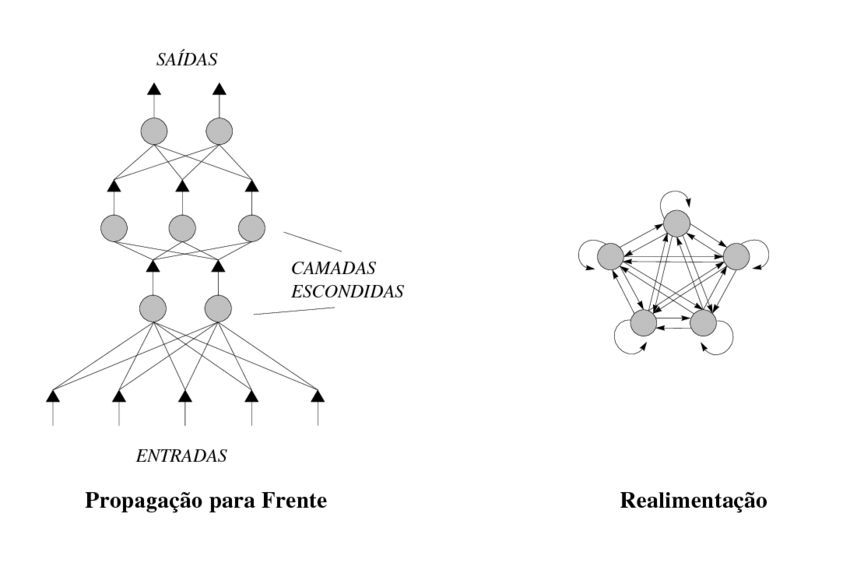
\includegraphics[scale=0.5]{img/graphNeuron2.png}
{\fontsize{11pt}{\baselineskip}\selectfont
\\Fonte: \cite{Rauber2005}
}
\end{figure}
 
Uma \textit{Feed-Forward Network} é uma rede multicamadas unidirecional, no qual não existe um ciclo entre as camadas de neurônios, ou seja, após o processamento de uma camada, as informações são sempre repassadas adiantes, para as sucessoras camadas, até a camada de saída, nunca sendo possível o retorno para camadas já executadas. Redes de propagação para frente, também chamadas de \textit{Multilayer Perceptron - MLP}, é a topologia de neurônios mais utilizada e estudada na área de aprendizado de máquina. As redes FFN são comumente aplicadas para o reconhecimento de padrões e classificação de dados.
 
Uma \textit{Recurrent Neural Networks} é uma rede que possui arestas entre os seus neurônios sem restrições, em que o comportamento dinâmico desempenha um papel fundamental nesse modelo. Em alguns casos, os valores de ativação da rede passam por um processo de relaxação, por múltiplos e até repetidos neurônios, até chegarem a um estado estável. Difere, principalmente, das redes FNN por possuir uma conexão com suas decisões passadas, em que cada saída pode ser tratada com uma nova entrada, armazenando conhecimento. É uma topologia poderosa e ao mesmo tempo complexa, tradicionalmente difícil de ser treinada. As redes RNN vêm sido aplicadas com grande sucesso para o processamento de linguagem natural, com ênfase em textos e falas.

Uma propriedade relevante das redes neurais é sua habilidade de aprender a partir do ambiente a qual foi inserida, também chamado de ambiente de aprendizado, em que sua capacidade de aprender é sucessivamente melhorada através do processo de adaptação dos parâmetros livres (pesos sinápticos e limiares) de sua rede. Este aprendizado pode ser adquirido de várias formas \citep{bishop2006pattern, duda1973pattern, Rauber2005}. Duas formas de aprendizado comuns são: aprendizagem supervisionada, em que o conhecimento é transmitido por meio de exemplos de entrada e saída; e aprendizagem não-supervisionada, no qual a rede só dispõem dos valores de entrada e deve descobrir as correlações entres os exemplos de treino.

Um método amplamente utilizado para o treinamento e aquisição de aprendizagem para redes FNN é o algoritmo de retro-propagação do erro (do inglês: \textit{Backpropagation}) proposto por \cite{werbos1974beyond}, baseado na regra de aprendizagem por correção de erro. Neste algoritmo (ilustrado na Figura \ref{fig:backpropagationExample}), a aprendizagem se consiste em dois passos através das diferentes camadas da rede: um passo para frente (propagação), no qual os pesos sinápticos da rede estão fixos, repassando os sinais funcionais normalmente desde a entrada até a saída; e um passo para trás (retro-propagação), em que cada saída gerada por um neurônio é subtraída da resposta real da rede, produzindo assim um sinal de erro, propagado em direção inversa as arestas da rede. O objetivo desse algoritmo é ajustar os pesos sinápticos da rede de forma que, a resposta real obtida, se aproxime ao máximo da desejada, ou seja, minimizar o erro gerado pela processamento da rede.

\begin{figure}[ht!]
\caption{Algoritmo \textit{Backpropagation} para treinamento de redes \textit{Feed-Forward Network}}
\label{fig:backpropagationExample}
\centering
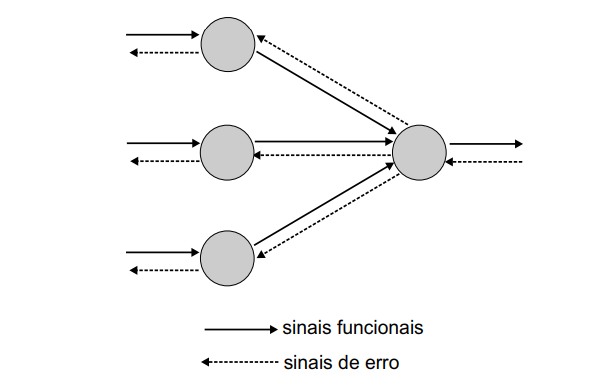
\includegraphics[scale=0.75]{img/backpropagationExample.png}
\end{figure}

Já para treinar uma rede RNN, o algoritmo de treinamento é baseado no \textit{Backpropagation}, chamado de \textit{Backpropagation Through Time - BPTT}. Que assim como o seu primitivo, calcula o erro gerado por cada neurônio, adaptando os pesos sinápticos. Como diferencial, a variável tempo é adicionada a cada passo. O que em prática significa, que para cada vez que é executado a retro-propagação do erro, uma camada cópia é gerada e deverá ser levada em consideração no próximo passo. Este algoritmo tende a ser computacionalmente custoso para cada novo passo dado, devido ao fato da ordem do erro aumentar a cada execução. Podendo reduzir os valores dos pesos a zero, como também crescerem exponencialmente, resultando em uma aprendizado lerdo e sujeito a ruído. Uma solução alternativa para este problema é o algoritmo aproximado \textit{Truncated BPTT}, no qual um limite de passos a serem considerados é definido, reduzindo assim o custo total de computação para sequências longas.
 
Por ser uma ferramenta poderosa, flexível e possuir uma grande capacidade de processamento, vem apresentando resultados excepcionais nas mais diversas aplicações da literatura \citep{gupta2018text, martin2018speech, bishop2006pattern, duda1973pattern, Rauber2005}, justificando assim a sua escolha como classificador de dados para este trabalho. 

Por outro lado, devido a sua complexidade e alto custo computacional, pode ser um obstáculo a ser enfrentado. Supondo que existam $n$ exemplos de teste, com $m$ características, $k$ \textit{Hidden layers}, no qual cada uma contém $h$ neurônios e existam $p$ neurônios de saída. O tempo total de execução do algoritmo de \textit{Backpropagation} para uma MLP seria $\mathcal{O}(n*m*h^{k}*p*i)$, no qual $i$ é o número de iterações executadas.

\subsection{K-vizinhos mais próximos}
O algoritmo K-vizinhos mais próximos (do inglês: \textit{K-neareast neighbours} - KNN) tem como objetivo determinar o rótulo de classificação de uma amostra, baseando-se em outras amostras vizinhas, advindas de um conjunto de treinamento. O classificador KNN, um dois mais simples e, ao mesmo tempo, um dos mais eficazes, dentre os algoritmos de classificação, é baseado em instâncias. Esse algoritmo encontra os $k$ objetos mais similares ao termo de consulta e realiza uma votação de acordo com as classes às quais pertencem esses $k$ objetos, assinalando por fim, uma classe ao objeto de teste. A literatura apresenta diversas formas para expressar essa distância/similaridade dentre os objetos de análise \citep{fukunaga1975knn, duda1973pattern}. Por exemplo, se os dados trabalhados estão em formato de texto, é comum utilizar a similaridade por cossenos. Por outro lado, se os dados possuírem formato numérico, possivelmente a distância euclidiana será mais eficaz.

\begin{figure}[ht!]
\caption{Ilustração do algoritmo K-vizinhos mais próximos aplicado em um plano cartesiano}
\label{fig:knnExample}
\centering
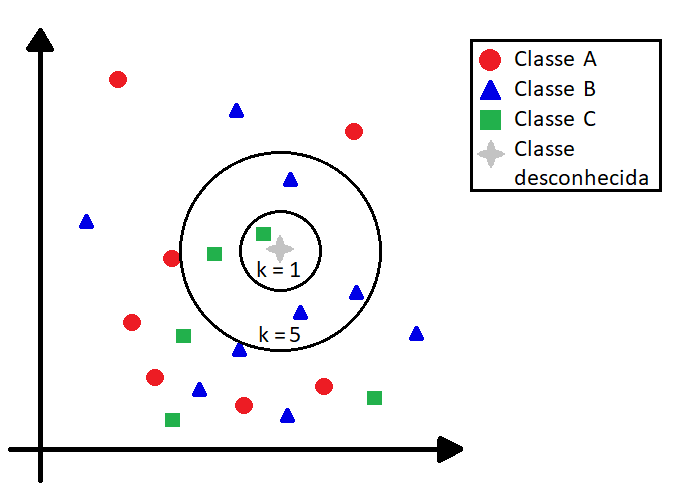
\includegraphics[scale=0.5]{img/knnExample.png}
{\fontsize{11pt}{\baselineskip}\selectfont
\\Fonte: Elaborado pelo autor
}
\end{figure}

Na Figura \ref{fig:knnExample}, é ilustrado o processo de classificação com o algoritmo KNN. Neste exemplo, têm-se três classes, anteriormente conhecidas, sendo elas: classe A (círculo vermelho), classe B (triangulo azul) e classe C (quadrado verde). O objetivo é identificar, por similaridade, a qual classe pertence a amostra (estrela cinza), olhando para o seus $k$ vizinhos mais próximos. Para $k = 1$, esse algoritmo classificaria a amostra como pertencente a classe C. Por outro lado, se o valor escolhido para $k$ é $5$, por votação majoritária, a amostra seria classificada como pertencente a classe B.

Um grande fator que pode definir a eficácia do algoritmo KNN no contexto em que é aplicado, é o valor de escolha para o $k$. Por ser um valor variável (não constante), deve ser determinado de forma empírica, variando de acordo com a base de dados. Caso o valor escolhido para $k$ seja muito baixo, a classificação ficará sujeita a \textit{outliers}, ou seja, dados atípicos ou ruídos, que não condizem com o contexto da classificação. Já por outro lado, se $k$ assumir um valor alto, a vizinhança poderá incluir elementos pertencentes a outras classes, não necessariamente relevantes ao objeto de análise, interferindo assim, no resultado final da rotulação \citep{fukunaga1975knn}. Por ser um fator relevante, deverá ser avaliado cuidadosamente.



\section{Privacidade dos dados e ética}
Das bases de dados sobre chamados emergenciais disponíveis, os conteúdos apresentam-se limitados, ou seja, com poucas informações, o que pode dificultar as pesquisas sobre o tema. Tal limitação denota  especialmente no aspecto à privacidade dos dados, uma vez que, por serem sigilosos, não podem ser compartilhados de forma a expor os indivíduos envolvidos.

A garantia da preservação do segredo das informações, além de uma obrigação legal contida na maioria dos Códigos de Ética profissional e também no Código Penal Brasileiro \citep{cp340}, é um dever \textit{prima facie}\footnote{que se pode constatar de imediato, sem ser necessário examinar melhor; claro, evidente, óbvio.} de todos e para com todos. Além do conteúdo sigiloso presente, faz-se necessário a efetivação de uma etapa referente a Ética:

\renewenvironment{quote}[1][1em]
  {\begin{adjustwidth}{#1}{0}}
  {\end{adjustwidth}}
\begin{quote}[4cm]
\begin{singlespace}
{\footnotesize  
Nas atividades de pesquisa, muitas vezes são utilizados dados constantes em prontuários e bases de dados. Essa utilização deve ser resguardada e permitida apenas para projetos previamente aprovados por um Comitê de Ética em Pesquisa, desde que plenamente descaracterizada a identificação do paciente, inclusive quanto as suas iniciais e registro hospitalar. Mesmo nas publicações científicas não deve ser possível identificar os pacientes através de fotografias ou outras imagens. Em caso de necessidade imperiosa, isto será permitido apenas com o consentimento, por escrito, dos mesmos o que possui amparo na própria Constituição Federal, em seu Art. 5º, item X. \citep{francisconi1998aspectos}.
}
\end{singlespace}
\end{quote}

Entretanto, como apontado por \cite{francisconi1998aspectos}, existem situações que claramente constituem exceções à preservação de segredos, devido ao risco de vida associado ou ao benefício social que pode ser obtido. Se tratando de uma área com poucas pesquisas realizadas, existem poucos resultados que comprovem a possível eficácia de um sistema que solucione a identificação correta de chamadas falsas em serviços de emergência. Consequentemente, os gestores que administram tais dados se sentem menos propensos a contribuir com pesquisas, por desconhecer o potencial que tais ferramentas poderiam oferecer ao processo.

Em suma, é fundamental compreender, respeitar e tratar com o devido cuidado, todas as informações dos usuários desses serviços emergenciais, como também, a necessidade de desenvolvimento de estratégias para tratar-las de forma eticamente adequada.
\chapter{Trabalhos Relacionados}
Neste capítulo, será apresentado trabalhos e pesquisas existentes na área que visão solucionar parcialmente ou completamente o problema de identificação de chamadas emergenciais falsas. Um trabalho soluciona parcialmente o problema, se o mesmo dispor alguma metodologia útil para resolver o problema geral. Como por exemplo técnicas de classificação de dados eficientes para texto, ou algum processamento de linguagem natural que facilite a seleção das características relevantes. Primeiramente apresenta-se ...

\section{Classificadores de texto}
Algoritmos de classificação de texto vêm sidos aplicados com sucesso em vários diferentes problemas e em diversas áreas de atuação e interesse, tais como rotulação de conteúdos, produtos, multimédia; Gerenciamento de Relacionamento com o Cliente (do inglês: \textit{Customer Relationship Management} - CRM) para empresas; monitoramento de conteúdo e tendências em redes sociais, dentre outros \citep{uysal2012novel, gupta2018text}. Alguns exemplos desses algoritmos são: Árvore de decisão, Máquina de Vetores de Suporte (do inglês: \textit{Support Vector Machine} - SVM), RNA e KNN.

Em uma consulta preliminar na literatura disponível, não foram identificados trabalhos e pesquisas que utilizem de algoritmos de classificação de texto para identificação de chamados falsos. Portanto, uma revisão dos principais algoritmos de classificação de texto aplicados a outros contextos é feita a seguir.

\cite{uysal2012novel} propuseram uma nova metodologia para extração de características em bases de dados textuais. E com o objetivo de avaliar a eficácia do novo método, executaram uma sequência de testes em quatro diferentes bases de dados, contendo estas diferentes características, com diferentes medidas de avaliação, junto ao uso de algoritmos de categorização de texto, como Árvore de decisão, SVM e RNA. Os resultados desse novo método foram promissores, apresentando alto índice de acurácia e o menor tempo de execução dentre os outros métodos de extração de características comparados. Dentre os resultados obtidos, os métodos RNA e SVM se destacaram diante à Árvore de decisão em quase todos os testes, com taxas de precisão superiores a $90\%$. Mais precisamente, o método RNA apresentou melhores resultados quando foi aplicado junto as bases de dados de \textit{e-mail spam} e textos \textit{Short Message Service} (SMS). Ressaltando assim, o potencial e a eficácia do uso da RNA para interpretação de linguagem natural.

O uso do SVM para classificação de texto foi proposto por \cite{joachims1998text}. Em sua publicação, Joachims identificou que os textos em geral possuem: um alto volume de dados, com várias características distintas; baixo índice de características irrelevantes ou inúteis para serem eliminadas; e são linearmente separáveis. Analisando essas características ele deduziu que, qualquer algoritmo de classificação que trabalhe bem nessas circunstâncias, também conseguiria classificar eficientemente um texto. E para validar sua hipótese, Joachims experimentou a eficácia do algoritmo SVM para classificação de texto utilizando as bases de dados ModApte e Ohsumed \textit{corpus}, quando comparado ao lado de métodos, até então, consolidados na literatura, como Naive Bayes, algoritmo de Rocchio, KNN e C4.5. Como resultados do experimento, obteve-se sucesso, visto que em média, o SVM acertou corretamente o \textit{target} em $86\%$ dos testes, superando todos os outros. Mais precisamente: Bayes ($72\%$), Rocchio ($79,9\%$), C4.5 ($79.4\%$) e KNN ($82.3\%$).

\section{Chamadas emergenciais falsas: Problemas e Soluções}
Chamadas emergenciais falsas são consideradas um fardo para os serviços emergenciais. Tais chamadas são responsáveis por perda de tempo, esforço, energia, recursos, enfim um bônus para o Estado.

Segundo \cite{waseem2010prank}, em uma análise feita sobre os dados das chamadas emergenciais recebidas entre outubro de 2004 e Maio de 2010, em Punjab, Paquistão, realçou que $97,85\%$ foram identificadas como falsas, onde, mais precisamente, $91,5\%$ destas foram identificadas como trote (brincadeiras ou insultos ao atendente); $7,27\%$ por busca de informações não relacionadas ao serviço; $1,5\%$ de chamadas por engano (discagem de número errado); e $0,14\%$ de chamadas onde o solicitante forjou a necessidade de um atendimento emergencial. 
Diante do exposto, ações foram efetivadas: a implantação de um sistema de monitoramento de chamadas e um sistema de bloqueio de chamadas, no qual após três ou quatro chamadas falsas ou trotes originadas do mesmo número, o bloqueio da linha telefônica seria realizado, impossibilitando assim, a efetuação de chamadas temporariamente.
Entretanto, observa-se que as medidas propostas não obtiveram grande êxito, uma vez que não houve redução significativa da incidência dessas chamadas indevidas.

\cite{rashford2010optimizing}, destacam a importância da otimização e do uso apropriado do sistema de chamadas emergenciais, combatendo os falsos chamados. Os autores realçam o desgaste financeiro que tal prática resulta na sociedade, retirando recursos que poderiam ser aproveitados em pacientes que realmente necessitam desse atendimento e transporte. Como medida preventiva, campanhas públicas de conscientização foram elaboradas, mas novamente não obtiveram os resultados esperados. Resultando assim, a introdução de penas mais severas, na legislação vigente da Austrália,  para quem realizasse falsos chamados, podendo ser multado em até \$ 10.000 ou 1 ano de prisão. 
Ainda sobre a descrição dos serviços de ambulância no referido país, é relatado o uso do Sistema de Prioridades para Despacho Médico (do inglês: \textit{Medical Priority Dispatch System} - MPDS). Neste sistema, o atendente é orientado a efetuar uma série de perguntas ao solicitante, com o objetivo de obter uma melhor descrição da emergência. Após essa triagem primária, a situação é então manualmente classificada em um código alfanumérico previamente definido, composto por: um número, entre 1 a 33 (Tabela \ref{tab:mpdsCodes}), que descreve o principal sintoma identificado; uma letra, \textit{Alpha}, \textit{Beta}, \textit{Charlie}, \textit{Echo} ou \textit{Omega}, que classifica a prioridade da emergência; e por fim, um outro número, que procura especificar ainda mais o problema.
Este método, bem como outros métodos similares, foram elaborados com o objetivo de alcançar um padrão comum, reduzindo o critério subjetivo e pessoal dos atendentes sobre a situação do paciente. Há dados que denotam a eficiência destes métodos, onde é possível obter mais informações sobre o estado do paciente, aumentando assim a chance de sobrevivência, prestando um atendimento mais específico e eficiente \citep{gray2008ampds}.

Os estudiosos relatam ainda que as chamadas menos prioritárias devem ainda passar por uma segunda triagem, sendo esta, por médicos especialistas, com o objetivo de um diagnóstico mais preciso. Sendo possível, mudar o prognóstico anterior, aumentando o nível de prioridade ou até mesmo não efetivando o despacho da ambulância ao local e sim o desencadeamento de medidas alternativas para o atendimento \citep{marks2002emergency, gray2008ampds}. Embora que é demonstrado alguma eficiência e otimização no processo, tais métodos ainda são efetuados manualmente pelos operadores. Não sendo aproveitado assim, do uso de ferramentas computacionais que automatizem e facilitem este processo.

\begin{table}[ht!]
\caption{Lista de códigos traduzidos do MPDS.}
\label{tab:mpdsCodes}
\centering
%\resizebox{\textwidth}{!}{%
\begin{tabular}{@{}clcl@{}}
\toprule
\multicolumn{4}{c}{\textbf{Códigos MPDS}}                                        \\ \midrule
1  & Dor abdominal                         & 18 & Dor de cabeça             \\ \midrule
2  & Reação alérgica                       & 19 & Problema no coração       \\ \midrule
3  & Mordida por animal                    & 20 & Exposição a calor ou frio \\ \midrule
4  & Assalto                               & 21 & Hemorragia                \\ \midrule
5  & Dor nas costas                        & 22 & Acidente industrial       \\ \midrule
6  & Dificuldade para respirar             & 23 & Overdose                  \\ \midrule
7  & Queimadura                            & 24 & Gravidez                  \\ \midrule
8  & Exposição a elemento químico perigoso & 25 & Problema psiquiátrico     \\ \midrule
9  & Ataque cardíaco                       & 26 & Doença                    \\ \midrule
10 & Dor no peito                          & 27 & Esfaqueamento ou tiro     \\ \midrule
11 & Asfixia                               & 28 & Acidente vascular         \\ \midrule
12 & Convulsão                             & 29 & Acidente de trânsito      \\ \midrule
13 & Diabete                               & 30 & Traumatismo               \\ \midrule
14 & Afogamento                            & 31 & Indivíduo inconsciente    \\ \midrule
15 & Eletrocussão                          & 32 & Sintoma não identificado  \\ \midrule
16 & Problema ocular                       & 33 & Cuidado paliativo         \\ \midrule
17 & Queda                                 &    &                           \\ \bottomrule
\end{tabular}%
\end{table}

Devido ao alto índice de trotes recebidos por serviços de telefonia mundial, tal como o serviço de Operador de Chamadas Internacionais (do inglês: International Operator Direct Calling - IODC), que têm como função conectar um turista em um viagem internacional, através de uma chamada, com um atendente de seu país natal. \cite{kuroiwa2004automatic} propuseram um sistema de identificação automática de trotes e chamadas falsas, baseado na tecnologia de reconhecimento de fala. Esse sistema foi desenvolvido para operar com base em ligações para o Japão, onde é verificado se a pessoa que deseja utilizar do serviço, compreende bem o idioma japonês. O teste é validado solicitando o usuário a repetir uma palavra em japonês, esperando um determinado tempo pela pronuncia. Caso o usuário pronuncie corretamente a palavra, pressupõem-se que o mesmo conhece o dialeto da região o qual está telefonando, portanto as chances de ser uma ligação real são altas, sendo assim, o usuário é rapidamente redirecionado para o atendente. Caso contrário, uma segunda e última tentativa de pronuncia é solicitada ao usuário. Se o mesmo errar ou não pronunciar a palavra, um aviso é dado e a ligação é encerrada. Como resultados da metodologia proposta, os autores informaram que depois de analisar cerca de $100.000$ chamadas, um total de $9489$ foram identificadas como chamadas reais, apresentando uma taxa de acerto de $97\%$ e um taxa de rejeição de chamadas falsas de $93\%$. O volume de trotes eram tão alto que houve dias na semana em que a quantidade ultrapassava $6.000$ de ligações rejeitadas. Contudo, apesar dos ótimos resultados apresentados pelos autores, esta aplicação é restrita ao contexto de chamadas internacionais e, ainda mais precisamente, específica e possível de ser implantada somente em alguns países, tal como o Japão, onde foi conduzido o estudo. Neste sentido, carece ainda o uso de uma ferramenta automatizada para ser aplicada no contexto do Brasil, por exemplo.

\section{Privacidade dos dados e ética}
Das bases de dados disponíveis, os conteúdos apresentam-se limitados, ou seja, com poucas informações, o que pode dificultar as pesquisas sobre o tema. Tal limitação denota  especialmente no aspecto à privacidade dos dados, uma vez que, por serem sigilosos, não podem ser compartilhados de forma a expor os indivíduos envolvidos.

A garantia da preservação do segredo das informações, além de uma obrigação legal contida na maioria dos Códigos de Ética profissional e também no Código Penal Brasileiro \citep{cp340}, é um dever \textit{prima facie} de todos e para com todos. Além do conteúdo sigiloso presente, faz-se necessário a efetivação de uma etapa referente a Ética:

\renewenvironment{quote}[1][1em]
  {\begin{adjustwidth}{#1}{0}}
  {\end{adjustwidth}}
\begin{quote}[4cm]
\begin{singlespace}
{\footnotesize  
Nas atividades de pesquisa, muitas vezes são utilizados dados constantes em prontuários e bases de dados. Essa utilização deve ser resguardada e permitida apenas para projetos previamente aprovados por um Comitê de Ética em Pesquisa, desde que plenamente descaracterizada a identificação do paciente, inclusive quanto as suas iniciais e registro hospitalar. Mesmo nas publicações científicas não deve ser possível identificar os pacientes através de fotografias ou outras imagens. Em caso de necessidade imperiosa, isto será permitido apenas com o consentimento, por escrito, dos mesmos o que possui amparo na própria Constituição Federal, em seu Art. 5º, item X. \citep{francisconi1998aspectos}.
}
\end{singlespace}
\end{quote}

Entretanto como apontado por \cite{francisconi1998aspectos}, existem situações que claramente constituem exceções à preservação de segredos, devido ao risco de vida associado ou ao benefício social que pode ser obtido. Se tratando de uma área com poucas pesquisas realizadas, existem poucos resultados que comprovem a possível eficácia de um sistema que solucione a identificação correta de chamadas falsas em serviços de emergência. E consequentemente, os gestores que administram tais dados se sentem menos propensos a contribuir com pesquisas, por desconhecer o potencial que tais ferramentas poderiam oferecer ao processo.

Em suma, é fundamental compreender o respeito e o devido cuidado que todas as informações dos usuários desses serviços emergenciais merecem, como também o desenvolvimento de estratégias para tratar-las de forma eticamente adequada.
\chapter{Metodologia}

\section{Base de dados}
A base de dados a ser trabalhada neste projeto é a \textit{Call Data}, do centro de comunicações do departamento de polícia de Seattle (\textit{Seattle Police Department Communications Center} - SPD), dos Estados Unidos da América. Esta base de dados representa os relatórios das chamadas emergenciais originados pela comunidade local, onde é armazenado cerca de $95\%$ de todos os chamados recebidos pelo departamento. No total, estão disponíveis 11 colunas de informações que descrevem a ocorrência (Tabela \ref{tab:callDataColumns}). Existindo mais de 3,9 milhões ocorrências únicas registradas desde 6 de fevereiro de 2009. Novos dados são inseridos diariamente pela equipe administradora, o que é um ponto positivo, pois é possível estimar o número de chamadas falsas recebidas em relação ao número total de chamados nos últimos anos, como também validar os objetivos ressaltados neste trabalho no cenário atual.

\begin{table}[ht!]
\caption{Tabela de atributos que descrevem uma ocorrência.}
\label{tab:callDataColumns}
\centering
\resizebox{\textwidth}{!}{%
\begin{tabular}{@{}llc@{}}
\toprule
\multicolumn{1}{c}{\textbf{Atributo}} & \multicolumn{1}{c}{\textbf{Descrição}}                           & \textbf{Formato} \\ \midrule
ID                                    & Identificador único                                              & Texto         \\ \midrule
Registro                              & Como foi resolvido o chamado                                     & Texto         \\ \midrule
Chamada                       & Origem da chamada (telefone, 911, alarme)                                               & Texto         \\ \midrule
Prioridade                            & Prioridade assimilada ao chamado                                 & Texto         \\ \midrule
Classificação inicial                 & Como foi classificado inicialmente a ocorrência                  & Texto         \\ \midrule
Classificação final                   & Como foi classificada pós o acompanhamento                         & Texto         \\ \midrule
Data e hora                           & Data e hora em que foi recebida o chamado                        & Data e hora   \\ \midrule
Tempo de chegada                      & Tempo de chegada do primeiro policial ao local do registro & Texto         \\ \midrule
Ponto cardeal                         & Ponto cardeal em relação ao mapa geográfico da cidade            & Texto         \\ \midrule
Setor                                 & Setor do ponto cardeal da ocorrência                             & Texto         \\ \midrule
Quadra                                & Quadra do setor da ocorrência                                    & Texto         \\ \bottomrule
\end{tabular}%
}
\end{table}

Por se tratar de uma base de dados pública e disponível na internet, as informações disponíveis são restritas em relação aos dados originais que são coletados diariamente pelo departamento, pois devido a sua natureza, são informações sigilosas e privadas da comunidade local. Dados como: nome, idade, sexo ou logradouro da ocorrência, foram removidos pelos administradores com o objetivo de preservar a privacidade dos envolvidos. 

Outra característica dessa base de dados é que ela está disponível no idioma inglês e com informações e relatórios dos chamados já bem resumidos, o que não possibilita tanta exploração e uso de algoritmos de processamento de linguagem natural. Contudo, como toda base de dados, um pré-processamento é necessário, com objetivo de eliminar ou corrigir erros de ortografia ou informações inconsistentes.
\section{Cronograma}

% Aqui vem a parte da bibliografia: use o comando \ppgccbibliography indicando
% apenas o nome do arquivo .bib (sem a extensão).
\ppgccbibliography{6-bibfile}
%\printbibliography

% Este comando encapsula o conjunto de anexos. A sua função é fazer com que a
% numeração dos anexos seja feita com letras maiúsculas (A, B, C, etc.) e a
% palavra "Anexo" anteceda as entradas no Sumário.
%\begin{attachments}
%\input{AnexoA}
%\end{attachments} % Fim dos anexos (usar apenas depois do último anexo)


\end{document}
